%; whizzy paragraph -pdf xpdf -latex ./whizzypdfptex.sh
%; whizzy-paragraph "^\\\\begin{frame}\\|\\\\emtext"
% latex beamer presentation.
% platex, latex-beamer でコンパイルすることを想定。 

%     Tokyo Debian Meeting resources
%     Copyright (C) 2012 Junichi Uekawa
%     Copyright (C) 2016 Nobuhiro Iwamatsu

%     This program is free software; you can redistribute it and/or modify
%     it under the terms of the GNU General Public License as published by
%     the Free Software Foundation; either version 2 of the License, or
%     (at your option) any later version.

%     This program is distributed in the hope that it will be useful,
%     but WITHOUT ANY WARRANTY; without even the implied warreanty of
%     MERCHANTABILITY or FITNESS FOR A PARTICULAR PURPOSE.  See the
%     GNU General Public License for more details.

%     You should have received a copy of the GNU General Public License
%     along with this program; if not, write to the Free Software
%     Foundation, Inc., 51 Franklin St, Fifth Floor, Boston, MA  02110-1301 USA

\documentclass[cjk,dvipdfmx,12pt]{beamer}
\usetheme{Tokyo}
\usepackage{monthlypresentation}

%  preview (shell-command (concat "evince " (replace-regexp-in-string "tex$" "pdf"(buffer-file-name)) "&")) 
%  presentation (shell-command (concat "xpdf -fullscreen " (replace-regexp-in-string "tex$" "pdf"(buffer-file-name)) "&"))
%  presentation (shell-command (concat "evince " (replace-regexp-in-string "tex$" "pdf"(buffer-file-name)) "&"))

%http://www.naney.org/diki/dk/hyperref.html
%日本語EUC系環境の時
\AtBeginDvi{\special{pdf:tounicode EUC-UCS2}}
%シフトJIS系環境の時
%\AtBeginDvi{\special{pdf:tounicode 90ms-RKSJ-UCS2}}

\newenvironment{commandlinesmall}%
{\VerbatimEnvironment
  \begin{Sbox}\begin{minipage}{1.0\hsize}\begin{fontsize}{8}{8} \begin{BVerbatim}}%
{\end{BVerbatim}\end{fontsize}\end{minipage}\end{Sbox}
  \setlength{\fboxsep}{8pt}
% start on a new paragraph

\vspace{6pt}% skip before
\fcolorbox{dancerdarkblue}{dancerlightblue}{\TheSbox}

\vspace{6pt}% skip after
}
%end of commandlinesmall

\title{Debian Update\\OSC 2019 Hokkaido}
\subtitle{Debian JP Project/東京エリアDebian勉強会\\出張版}
\author{杉本 典充\\ dictoss@debian.or.jp}
\date{2019年6月1日}
\logo{
\includegraphics[width=8cm]{image200607/openlogo-light.eps}}

\begin{document}

\section{表紙}

\begin{frame}
\titlepage{}
\end{frame}

\section{目次}

\begin{frame}{Agenda}
  \begin{itemize}
  \item Debian とは?
  \item Debian JP Project と Debian 勉強会
  \item Debian 10 (Buster)
  \item Debian Updates
  \item 今後のイベント
  \end{itemize}
\end{frame}

%-------------------

\section{Debian とは?}

\begin{frame}\begin{center}\Huge{Debian とは?}\end{center}\end{frame}


\begin{frame}{Debian とは?}

{\color{red}{フリー/オープン}}な{\color{red}{ユニバーサル}}オペレーティングシステム を作成しようとするボランティアベースのプロジェクト

\begin{table}[htb]
  \begin{tabular}{|c|c|c|}
    \hline
    ディストリ & 企業 & ボランティア \\ \hline
    Fedora & RedHat支援あり & あり  \\ \hline
    RHEL & RedHat & なし  \\ \hline
    CentOS & RedHat支援あり & あり \\ \hline
    \color{red}{Debian}  & \color{red}{なし} & \color{red}{あり} \\ \hline
    Ubuntu  & Canonical & あり \\ \hline
    openSUSE & SUSE支援あり & あり \\ \hline
    SLES & SUSE & なし \\ \hline
  \end{tabular}
\end{table}

\end{frame}

\begin{frame}{Debian とは?}
  世界規模で開発が行われており、63ヶ国、約1,100名\footnote{\url{https://db.debian.org/}}のDebian公式開発者が開発を行っている。
  パッケージメンテナや翻訳などの貢献者も入れるともっと多くの開発者が参加していることになる。
 \begin{center}
%%%   \includegraphics[width=0.7\hsize]{image201707/group_photo_t.jpg}
 \end{center}
\end{frame}


\begin{frame}{Debian とは?}

\begin{itemize}
  \item 様々な用途に使える汎用的な作り
    \begin{itemize}
    \item デスクトップPC、ノートPCなどの普段利用するコンピュータのOS
    \item Linuxサーバ (例:webサーバのシェア:\url{https://w3techs.com/technologies/details/os-linux/all/all})
    \item 組込デバイスのベースOS (多くのCPUで動作する)
  \end{itemize}
  \item 「Debian」ベースな派生OSの源流
  \begin{itemize}
    \item Ubuntu や Raspbian といったディストリビューションのベースはDebian
    \item 派生先のディストリビューションと相互に情報交換をして開発している
  \end{itemize}
\end{itemize}

\end{frame}


\begin{frame}{Debian とは?}

\begin{itemize}
  \item 2019年6月の時点で、最新版は {\color{red}{Debian 9.9}} (コードネーム: Stretch)
  \begin{itemize}
    \item パッケージ数は{\color{red}{約51000}}を提供
    \item 公式にサポートするCPUアーキテクチャは{\color{red}{10}}
  \end{itemize}
  \item {\color{red}{約2年毎}}にリリース
  \item 次のリリース Debian 10 (コードネーム: {\color{red}{}}Buster)は 2019年中頃にリリースすると思われる
  \item コードネームはトイ・ストーリーのキャラクターを採用
\end{itemize}

\end{frame}


\begin{frame}{Debian とは?}

\begin{itemize}
  \item Debian 社会契約
    \begin{itemize}
      \item \url{https://www.debian.org/social_contract.ja.html}
      \item Debian 開発者たちが目指すフリーソフトウェアコミュニティーの在り方
    \end{itemize}
  \item Debian フリーソフトウェアガイドライン(DFSG)
    \begin{itemize}
      \item Debian 社会契約の一部
      \item Debian が考えるフリーソフトウェアの定義
      \item オープンソースの定義のひな形にもなっている
    \end{itemize}
  \item Debian Policy
    \begin{itemize}
      \item \url{https://www.debian.org/doc/debian-policy/}
      \item Debian パッケージの区分、内容やルール、ファイル配置の方針を定義
    \end{itemize}
\end{itemize}

\end{frame}


\begin{frame}{Debian とは?}
まとめると
\begin{itemize}
  \item Debianはフリー/オープンなオペレーティングシステム (OS)を作成しようとするボランティアベースのプロジェクト
  \item 自分たちの考えるフリーという言葉に関する定義、開発目的、パッケージングポリシーを厳格に決めている
  \item 世界中に1,100人以上の開発者がおり、他のディストリビューションのベースとして採用されている
  \item 約2年毎にリリースが行われ、多くのパッケージとアーキテクチャをサポートしている
  \item 上記のような特徴から様々なところで利用されているLinuxディストリビューション
\end{itemize}

\end{frame}

%------------------


\section{Debian JP Project と Debian勉強会}


\begin{frame}
  \begin{center}\Huge{Debian JP Project\\と\\Debian勉強会}\end{center}
\end{frame}

\subsection{Debian JP Projectとは}
  
\begin{frame}{Debian JP Project とは?}

\begin{itemize}
  \item 日本でDebianを普及させることを目的とした任意団体
  \item 活動内容
  \begin{itemize}
    \item Debian の日本語による情報発信
    \item ユーザとの情報交換
    \item Debian 開発者、パッケージメンテナの育成など
  \end{itemize}
\end{itemize}

\end{frame}

\subsection{Debian勉強会}

\begin{frame}
  
\frametitle{Debian勉強会}
\begin{itemize}
 \item 2005年1月開始
 \item Debian Developer 上川さん発起人
 \item 東京と関西で月に一回コンスタントに開催しているDebian開発者、ユーザによる勉強会
 \item webサイト
   \begin{itemize}
   \item 東京エリアDebian勉強会 \url{https://tokyodebian-team.pages.debian.net/}
   \item 関西Debian勉強会 \url{https://wiki.debian.org/KansaiDebianMeeting}
   \end{itemize}
\end{itemize}

\end{frame}


\begin{frame}

\frametitle{Debian勉強会:解決したい内容}
\begin{itemize}
 \item<1-> 問題
       \begin{itemize}
	\item MLとIRCで情報交換していた
	\item face-to-faceであう場所がない
	\item まとまったドキュメントが出てこない
       \end{itemize}
 \item<2-> Debian勉強会の提案
       \begin{itemize}
	\item 定期的に集まる
	\item 資料を作成する。(GPLで!) \\
	  {\small \url{https://salsa.debian.org/tokyodebian-team/monthly-report}}
       \end{itemize}
\end{itemize}

\end{frame}


\subsection{最近の勉強会}


\begin{frame}
  
\frametitle{Debian勉強会:最近の勉強会}
  
\begin{itemize}
  \item Debian 界隈やパッケージング関連の話題など専門の人に話を聞く
  \item Debianで気になった事柄を調べてレポートする
  \item 前回の内容(東京 5月):
	\begin{itemize}
	\item 場所: 朝日ネットさん
    \item /usr Mergeについて(発表者:yy\_y\_ja\_jpさん)
    \item Hack Time
	\end{itemize}
  \item 各地のイベントでDebian普及活動
	\begin{itemize}
      \item OSC2018北海道、OSC2018京都、OSC2018福岡、OSC2019東京
      \item 関西オープンフォーラム
	  \item Debian/Ubuntu ユーザミートアップ in 札幌
	\end{itemize}
\end{itemize}

\end{frame}

%-----------------------

\section{次期安定版 Debian 10 (Buster)}

\begin{frame}
  \begin{center}\Huge{Debian 10 (Buster)\\Full freeze中\\リリースまであと少し!}\end{center}
\end{frame}


\begin{frame}{Debian 10 Buster}% [containsverbatim]

Debian 10 (コードネーム:Buster)

\begin{itemize}
\item 現在開発を進めている次の安定版リリース
\item Debianはtime-based freezeを採用しており、およそ2年毎のリリースを目指す
\end{itemize}
  \begin{center}
    %%% \includegraphics[width=0.6\hsize]{image201906/buster.jpg}
    % https://pixar.fandom.com/wiki/Buster
  \end{center}
\end{frame}


\subsection{リリースまでの流れ}

\begin{frame}{リリースまでの流れ}% [containsverbatim]

Debian 10のリリースまでの流れ \\
\url{https://wiki.debian.org/DebianBuster}
  
\begin{itemize}
\item 2019-01-12: Transition freeze
  \begin{itemize}
  \item これ以降、大規模な変更や他のパッケージに大きな影響を与える変更を行ってはいけない
  \end{itemize}
\item 2019-02-12: Soft freeze
  \begin{itemize}
  \item 変更は小規模で的を絞った内容に限って行う
  \item 例)バグ修正、セキュリティ修正、他のパッケージとの調整
  \item この期日までにtestingに移行していないパッケージは次のリリースに含まれません
  \end{itemize}
\item 2019-03-12: Full freeze ←今はこの段階
  \begin{itemize}
  \item unstableにアップロードしたパッケージをtestingに移行するにはリリースチームのレビューが必要
  \item debdiffを添えてunblockというバグ報告を行いレビューしてもらう
  \end{itemize}
\end{itemize}
\end{frame}


\begin{frame}{リリースまでの流れ}% [containsverbatim]

Debian 10 はいつリリースされるのか?

\begin{itemize}
\item Debianでは、リリースクリティカルバグ(RC bug)が 0 個になったときにリリースする
\item 【参考】 Debian 9 Stretch のリリース日は 2017/6/17
\item 現在のリリースクリティカルバグの一覧
  \begin{itemize}
  \item \url{https://bugs.debian.org/release-critical/}
  \end{itemize}
\end{itemize}

\begin{center}
  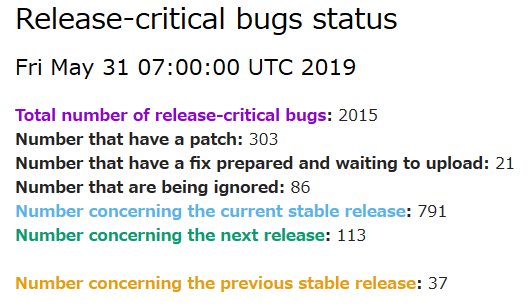
\includegraphics[width=0.45\hsize]{image201906/debian-rcbug-1_20190531.png}
  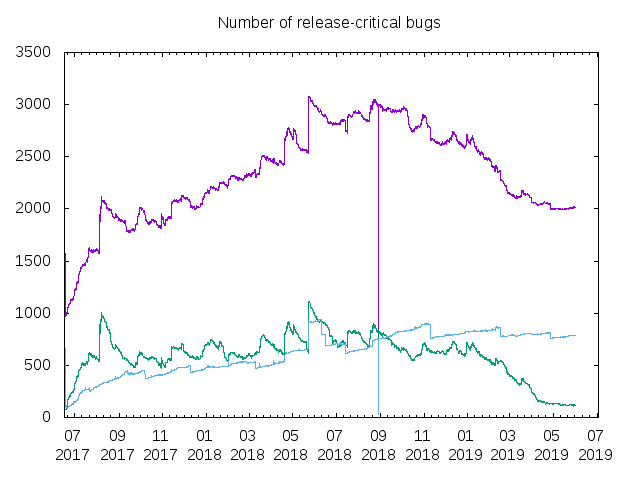
\includegraphics[width=0.45\hsize]{image201906/debian-rcbug-2_20190531.png}
  % https://bugs.debian.org/release-critical/
\end{center}

\end{frame}


\subsection{Debian 9 から Debian 10 の変更点}

\begin{frame}
  \begin{center}\Huge{Debian 9 から Debian 10の変更点}\end{center}
\end{frame}


\begin{frame}{Debian 9 から 10 の変更点}% [containsverbatim]

【ご注意ください】

まだリリースノートは確定していません。今後変わることがあります。

【作成中のリリースノート】

\url{https://www.debian.org/releases/buster/releasenotes}

\end{frame}


\subsection{テーマ}

\begin{frame}{テーマ}% [containsverbatim]

テーマはAlex Makasさん提案の「futurePrototype」に決定
  
\begin{center}
  
\includegraphics[width=0.75\hsize]{image201906/futurePrototype-wallpaper-1920x1080.png}
\end{center}

\url{https://bits.debian.org/tag/artwork.html}

\url{https://wiki.debian.org/DebianArt/Themes/futurePrototype}

\end{frame}


\subsection{アーキテクチャ}

\begin{frame}{アーキテクチャ}% [containsverbatim]

リリースするアーキテクチャは、Debian 9 Stretch と同じ予定(10つ)\footnote{\url{https://www.debian.org/releases/buster/amd64/release-notes/ch-whats-new.ja.html}}

\begin{itemize}
\item amd64, i386
\item arm64, armel, armhf
\item mips64el, mipsel, mips
\item ppc64el
\item s390x
\end{itemize}

\end{frame}


\subsection{提供ソフトウェアのバージョン}

\begin{frame}{提供ソフトウェアのバージョン}% [containsverbatim]

主要なソフトウェアは以下のバージョンを提供予定\footnote{\url{https://www.debian.org/releases/testing/amd64/release-notes/ch-whats-new.ja.html\#newdistro}}

\begin{itemize}
\item Linux カーネル 4.19
\item ツールチェイン(GCC 8.3/7.4, binutils 2.31.1, glibc 2.28), LLVM 7.0.1/6.0.1
\item Perl 5.28.1, Python 3.7.2/2.7.16, Ruby 2.5.1, PHP 7.3.4, Go 1.11.6, OpenJDK 11.0.3
\item GNOME 3.30, KDE 5.14.5.1, Cinnamon 3.8.8, MATE 1.20, Xfce 4.12.5, lxde 0.99.2, lxqt 0.14.1
\item MariaDB 10.3.14, PostgreSQL 11.3, sqlite 3.27.2/2.8.17 
\item OpenSSH 7.9p1, OpenSSL 1.1.1b, GnuPG 2.2.12/1.4.23
\item etc..
\end{itemize}

\end{frame}


\subsection{大きな新機能}

%% 第2章 Debian 10 の最新情報 から紹介
%% https://www.debian.org/releases/buster/amd64/release-notes/ch-whats-new.ja.html

\subsubsection{UEFI セキュアブートに対応}

%%% 2.2.1. UEFI Secure Boot

\begin{frame}{UEFI セキュアブートに対応}% [containsverbatim]

UEFI Secure Boot に対応
 
\begin{itemize}
\item UEFIの設定で Secure Boot が有効な状態でも、Debian 10 を起動できるようになった
\item shim-signed, grub-efi-\{amd64,ia32\}-signed, Debian 10 が提供する公式linuxカーネルパッケージ をインストールする必要がある
\item DKMSなどで独自ビルドしたkernel moduleはSecure Boot時に利用できない
\end{itemize}
    
\end{frame}


\subsubsection{AppArmor のデフォルト有効化}

%%% 2.2.2. AppArmor enabled per default

\begin{frame}{AppArmor のデフォルト有効化}% [containsverbatim]

AppArmor がインストール時にデフォルトで有効
 
\begin{itemize}
\item AppArmor とはマウント、ptrace、シグナルの権限、ファイルの読み書き実行などをプログラムごとに定義したプロファイルにしたがってアクセス制御を行う機能
\item 多くのプロファイルは apparmor-profiles-extra をインストールすると利用可能
\item AppArmor 自体は Debian 10 より前のバージョンでも提供していたが、デフォルトは無効であった
\end{itemize}
    
\end{frame}


\subsubsection{nftables のデフォルト化}

%%% 2.2.6. Network filtering based on nftables framework by default

\begin{frame}{nftables のデフォルト化}% [containsverbatim]

ネットワークフィルターの設定プログラムは nftables がデフォルト
  
\begin{itemize}
\item iptables を完全に置き換える目的で作られ、より高機能な nftables をデフォルトに変更
\item iptables コマンド は iptables-nft へのシンボリックリンク
\item 従来の iptables は iptables-legacy にコマンド名を変更して提供される
\end{itemize}
    
\end{frame}


\subsubsection{そのほかの新たな機能}

%%% 2.2.3. Optional hardening of APT
%%% 2.2.4. Unattended-upgrades for stable point releases
%%% 2.2.5. Substantially improved man pages for German speaking users
%%% 2.2.7. Cryptsetup defaults to on-disk LUKS2 format
%%% 2.2.8. driverless printing with CUPS 2.2.10
%%% 2.2.9. Basic support for Allwinner A64 based devices

\begin{frame}{そのほかの新たな機能}% [containsverbatim]

\begin{itemize}
\item Optional hardening of APT
\item Unattended-upgrades for stable point releases
\item Substantially improved man pages for German speaking users
\item Cryptsetup defaults to on-disk LUKS2 format
\item driverless printing with CUPS 2.2.10
\item Basic support for Allwinner A64 based devices
\end{itemize}
    
\end{frame}


\begin{frame}{Debian 9 から 10 の変更点}% [containsverbatim]

GNOME は Wayland での動作がデフォルトになりました

\begin{itemize}
\item 「GNOME on Xorg」も選べます
\item 他のデスクトップ環境は Xorg で動作します
%\item GNOME で Wayland を使う場合に日本語を入力できないことがある
%  \begin{itemize}
%  \item 日本語入力処理(Input Method)周りに問題が残っており、修正対応中
%  \end{itemize}
\end{itemize}

\begin{center}
  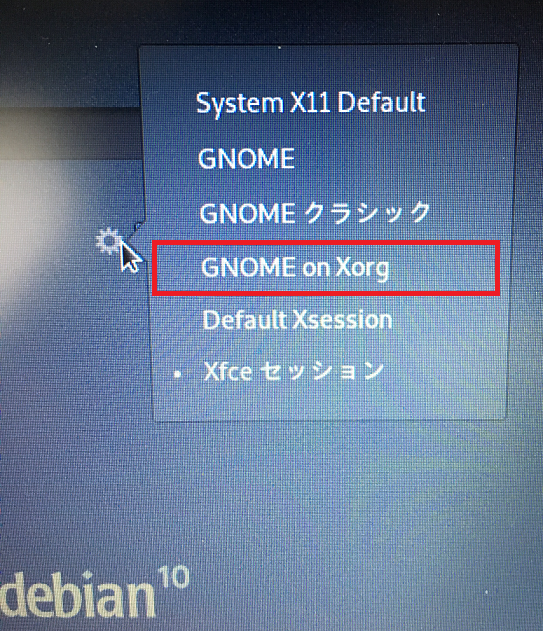
\includegraphics[width=0.5\hsize]{image201902/GDM_GNOME_select_mark.png}
\end{center}

\end{frame}


\begin{frame}{Debian 9 から 10 の変更点}% [containsverbatim]

  \begin{itemize}
  \item openssl-1.1.1 系の採用により TLSv1.3 が利用可能
  \item opensshにおいてSSH 1プロトコルは完全削除となったため、SSH 2プロトコルを利用すること
  \item glibc-2.28 を 採用しており linux カーネルの下限が 3.2 に変更
    \begin{itemize}
    \item 古いOS上でコンテナ環境を作っている場合、Debian 10 がコンテナで動かない場合あり
    \end{itemize}
  \end{itemize}

\end{frame}


\subsection{インストーラ}

\begin{frame}{インストーラ}% [containsverbatim]

Debian Installer Buster RC 1 Release

\begin{itemize}
  \item \url{https://www.debian.org/devel/debian-installer/News/2019/20190415}
  \item いち早くBusterを試してみたい方は以下からダウンロードしてインストールできます
  \begin{itemize}
    \item \url{https://www.debian.org/devel/debian-installer/index.ja.html}
  \end{itemize}
\end{itemize}

\end{frame}


\subsection{バグレポート}

\begin{frame}{バグレポートをお願いします}% [containsverbatim]
  \begin{itemize}
  %%%
  \item できればリリース前にインストールして使ってみていただきたいです
  %%%
  \item 何かおかしい動作や不具合を見つけた場合はバグレポートをお願いします
  \item バグレポートの仕方(レポートは英語で送る必要あり)
    \begin{itemize}
    \item \url{https://www.debian.org/Bugs/Reporting.ja.html}
    \end{itemize}
  \item バグレポートの前に少し相談してみたい方は、日本語のDebian JPメーリングリストや、SNSで相談してみてください
    \begin{itemize}
    \item \url{https://www.debian.or.jp/community/ml/openml.html}
    \item Twitter: @debian\_jp
    \end{itemize}
  \end{itemize}
\end{frame}

%-----------------------

\section{Debian Updates}

% 半年間の以下MLから抜粋して紹介する
%  https://lists.debian.org/debian-announce/
%  https://lists.debian.org/debian-devel-announce/

\begin{frame}
  \begin{center}\Huge{Debian Updates}\end{center}
\end{frame}


\subsection{released timeline}

\begin{frame}{Debian Updates}% [containsverbatim]

\begin{itemize}
  \item 2019/01/23:  Updated Debian 9.7  released
  \item 2019/02/16:  Updated Debian 9.8  released
  \item 2019/04/27:  Updated Debian 9.9  released
\end{itemize}

\end{frame}


\subsection{Debian 10 Buster release timeline}

\begin{frame}{Debian Updates}% [containsverbatim]

\begin{itemize}
  \item 2019/01/20: Bits from the Release Team: Debian 10 'buster' freeze has begun
  \item 2019/02/02: Debian Installer Buster Alpha 5 release
  \item 2019/02/12: Debian 10 'buster' is now in the soft freeze
  \item 2019/03/12: Debian 10 'buster' is frozen; let's get it in shape\footnote{\url{https://lists.debian.org/debian-devel-announce/2019/03/msg00003.html}}
  \item 2019/04/14: buster freeze update\footnote{\url{https://lists.debian.org/debian-devel-announce/2019/04/msg00003.html}}
    \begin{itemize}
      \item Debian 10 BusterでリリースするCPUアーキテクチャはDebian 9 Stretchと同じとすることに決定
    \end{itemize}
  \item 2019/04/15: Debian Installer Buster RC 1 release
\end{itemize}

\end{frame}


\subsection{Debian Project Leader Elections 2019}

\begin{frame}{Debian Updates}% [containsverbatim]

  \begin{itemize}
 
\item 2019/4/20: Debian Project Leader Elections 2019 投票締切
\item 2019年の Debian プロジェクトリーダー(DPL)を決める選挙を実施
\item Sam Hartman さんが選出
\item 選挙における声明は \url{https://www.debian.org/vote/2019/platforms/hartmans} を参照
\end{itemize}

\end{frame}


\subsection{Bits from the DPL / Bits from Debian}

\begin{frame}{Debian Updates}% [containsverbatim]

Bits from the DPL

\begin{itemize}
\item 月末頃に"debian-devel-announce@lists.debian.org"のMLにDebian Project Leaderがプロジェクトの進捗を報告している
\item 時間のない方でもこれを読んでおけばDebian Projectの大まかな動きがわかる
\end{itemize}

【お得な情報:Bits from Debian】

\begin{itemize}
\item \url{https://bits.debian.org/}
\item Debian の公式ブログ
\item ここをチェックしておけば、Debianのニュースが入ってきます
\end{itemize}

\end{frame}


\subsection{開発方針の議論}

\begin{frame}{Debian Updates}% [containsverbatim]

開発方針の議論
  
\begin{itemize}
\item 2019/03/05: TC decision on ``Merged /usr'' - \#914897\footnote{\url{https://lists.debian.org/debian-devel-announce/2019/03/msg00001.html}}
\item usr mergeとは、 /\{bin,sbin,lib\} を /usr/\{bin,sbin,lib\} へのシンボリックリンクにする話
\item Debian 10 Buster を新規インストールした場合は usr merge された状態になる
\item 議論の結果、従来の usr merge されていない環境もサポートすべきとの結論になった
\item Debian 11 Bullseye でさらに取り組みを進める
\end{itemize}

\end{frame}


\subsection{サーバ関連}

\begin{frame}{Debian Updates}% [containsverbatim]

ミラーサーバの古いバージョンの提供終了
  
\begin{itemize}
\item 2019/03/20: Removal of Wheezy and Jessie (except LTS) from mirrors\footnote{\url{https://lists.debian.org/debian-devel-announce/2019/03/msg00006.html}}
\end{itemize}

\end{frame}

\subsection{DebConf19}

\begin{frame}{Debian Updates}% [containsverbatim]

DebConf19関連
  
\begin{itemize}
\item 2019/03/21: Registration is now open for DebConf19, in Curitiba, Brazil\footnote{\url{https://lists.debian.org/debian-devel-announce/2019/03/msg00007.html}}
\item 2019/04/03: Share your plans for DebCamp19 Paulo Henrique de Lima Santana\footnote{\url{https://lists.debian.org/debian-devel-announce/2019/04/msg00000.html}}
\end{itemize}

\end{frame}



%-----------------------

\section{日本語によるDebianの情報}

\begin{frame}\begin{center}\Huge{日本語によるDebianの情報}\end{center}\end{frame}

\begin{frame}{日本語によるDebianの情報}
\begin{itemize}
  \item Debian JP Project \\
      \url{https://www.debian.or.jp}
  \item 東京エリアDebian勉強会\\
      \url{https://tokyodebian-team.pages.debian.net/}
  \item 関西Debian勉強会 \\
      \url{https://wiki.debian.org/KansaiDebianMeeting}
  \item Twitter \\
      \url{@debian_jp}
  \item  雑誌 Software Design 技術評論社発行 \\
    「Debian Hot Topics」(隔月連載)
\end{itemize}
\end{frame}

%----------------

\section{今後のイベント}

\begin{frame}\begin{center}\Huge{今後のイベント}\end{center}\end{frame}


\begin{frame}{今後のイベント}

\begin{itemize}
\item 6/15(土) 第175回東京エリアDebian勉強会(予定)
  \begin{itemize}
  \item \url{https://tokyodebian-team.pages.debian.net/2019-06.html}
  \end{itemize}
\item 6/23(日) 関西Debian勉強会(予定)
  \begin{itemize}
  \item \url{https://wiki.debian.org/KansaiDebianMeeting/20190623}
  \end{itemize}
\end{itemize}

\end{frame}

\end{document}

;;; Local Variables: ***
;;; outline-regexp: "\\([ 	]*\\\\\\(documentstyle\\|documentclass\\|emtext\\|section\\|begin{frame}\\)\\*?[ 	]*[[{]\\|[]+\\)" ***
;;; End: ***
